\begin{tikzpicture}[font=\scriptsize]
  \seqactor{0}{Exéc. Deliver}{AOe-sD1.12}
  \seqactor{4.2}{Pilote Deliver}{AOp-sD1}
  \seqactor{8.6}{Coordinator}{CA-sD1}
  \seqactor{12.6}{Tactical Deliver}{AT-sP4}
  \seqactor{17.0}{Strategic}{AS-sP1}

  \seqline{0}{9.6} \seqline{4.2}{9.6} \seqline{8.6}{9.6} \seqline{12.6}{9.6} \seqline{17.0}{9.6}

  \seqmsg{exec}{1.2}{0}{4.2}{\emph{DeliveryCompleted}}
  \seqmsg{report}{2.4}{4.2}{8.6}{\emph{OperationalReport}}
  \seqmsg{report}{3.6}{8.6}{12.6}{\emph{ProcessStatusReport}}
  \seqmsg{report}{4.8}{12.6}{17.0}{\emph{MacroProcessReport}}

  \seqnote{0}{6.0}{17cm}{Remontée hiérarchique REPORT, symétrique de la descente AMENDMENT (figure Architecture globale) :
   chaque niveau consolide l'information avant de la transmettre au niveau supérieur -- aucun saut de niveau
   observé dans le code.}
  \seqnote{0}{7.6}{17cm}{Confirmation client (\emph{OrderConfirmed}, via \emph{PromisedDeliveryDate} $\to$ \emph{OrderConfirmationOrder}
   $\to$ \emph{CustomerConfirmationTask}) est émise plus tôt dans le cycle, dès la date promise calculée --
   non répétée ici (voir figure Réception commande).}
\end{tikzpicture}
